% This file is part of the openLilyLib project
% Copyright Urs Liska 2013
% This file and the resulting PDF document aren't distributed under a free license.

\documentclass[DIV=12]{scrreprt}
\usepackage{plaintextGerman}
\usepackage{adjustbox}

\usepackage{pdfpages}

\begin{document}
\begin{center}
\vspace*{3cm}
{ \Huge \textbf{\textsf{LilyPond\\
\vspace{1ex}
\huge Partitur-Beispiele}} }

\bigskip
{ \Large Urs Liska }

\emph{September 2013} 

\end{center}

\vspace{2cm}

Als Anhang zu dem Textdokument \emph{Reintext-basiertes Arbeiten für Musikwissenschaftler} zeigen die folgenden Seiten Ausschnitte exemplarischer Partituren, die mit GNU LilyPond%
\footnote{\url{http://www.lilypond.org}}
gesetzt wurden.
Die Beispiele sind in zwei Gruppen gegliedert, die jeweils eigene Aspekte darstellen sollen:
\paragraph{Veröffentlichungsqualität}
Partituren, die mit mehr oder weniger großem Aufwand im Detail perfektioniert wurden.
Diese Beispiele zeigen, dass LilyPond professionellen verlegerischen Ansprüchen genügt.
Gleichzeitig weisen diese Beispiele auch eine große stilistische Bandbreite auf.

\paragraph{Standardqualität, mit oder ohne Stilvorlagen}
Partituren, die keine nennenswerten individuellen Anpassungen aufweisen.
Diese Beispiele sind daher repräsentativ für die Qualität der vorläufigen Ergebnisse und für das hohe Maß an Les- und Verwendbarkeit der Standardausgabe.
Auch wenn diese Beispiele je nach Komplexität teilweise recht weit von Publikationsqualität entfernt sind, zeigen sie, wie gut und weitgehend man diese Partituren im Arbeitsprozess verwenden kann, ohne sich um notentypografische Details kümmern zu müssen.
Einige Partituren entsprechen LilyPonds Standard-Erscheinungsbild, andere wurden mit Hilfe von Stilvorlagen verändert, ohne jedoch individuelle Satzkorrekturen aufzuweisen.

Einige der Ausschnitte sind urheberrechtlich geschützten Werken entnommen und nur für den Zweck der Demonstration zusammengestellt.
Bitte respektieren Sie dies und geben das Dokument nicht an Dritte weiter.

\pagebreak
\section*{Publikationsqualität}

\begin{itemize}
\item Oskar Fried: Sommernachtslied op. 7,\,Nr.\,4
\item Martin Anton Schmid: Achtsamkeit
\item Georg Muffat: Cor vigilans
\item Mike Solomon: Aux Eppes
\item Mike Solomon: Zauberbuch
\item Julio Sagreras: Gitarrenschule
\end{itemize}

\includepdf{images/publication/fried-7-4.pdf}
\includepdf{images/publication/achtsamkeit.pdf}
\includepdf[pages=2]{images/publication/muffat.pdf}
\includepdf[pages=8,angle=90]{images/publication/auxeppes.pdf}
\includepdf[pages=21,angle=90]{images/publication/zauberbuch.pdf}
\includepdf[pages=1]{images/publication/lecon.pdf}

\section*{Standard-Ausgabe}

\bigskip

\textbf{A) Partituren, deren Erscheinungsbild lediglich mit Hilfe von Stilvorlagen verändert wurde \\
(keine individuellen Satzkorrekturen):}

\begin{itemize}
\item Ludwig van Beethoven: Sonate op. 10,\,3
\item Josef Suk: Bagatella 
\item Franz Schubert: Seligkeit
\item Arnold Schönberg: Erhebung op. 2,\,3
\item Julio Sagreras: El colibri
\end{itemize}

\noindent\textbf{B) Partituren in LilyPonds Original-Erscheinungsbild \\
(keinerlei Korrekturen außer Seitenlayout und evtl. pauschaler Notensystemgröße):}

\begin{itemize}
\item Arnold Schönberg: Gethsemane
\item Alban Berg: Orchesterstück op. 6,\,1 (achthändige Bearbeitung)
\item Bryan Ferneyhough: La Chute d'Icare
\item Arnold Schönberg: Nie werd ich, Herrin, müd op. 8.\,4 (Klavierauszug)\\
Vergleich Standardausgabe von LilyPond und Finale
\end{itemize}

\includepdf[pages=1]{images/default/beethoven.pdf}
\includepdf[pages=1]{images/default/bagatella.pdf}
\includepdf[pages=1]{images/default/seligkeit.pdf}
\includepdf[pages=1]{images/default/erhebung.pdf}
\includepdf[pages=1]{images/default/colibri.pdf}
\includepdf[pages=1]{images/default/gethsemane.pdf}
\includepdf[pages=1]{images/default/berg.pdf}
\includepdf[pages=1]{images/default/ferneyII.pdf}


\includegraphics[max width=\textwidth]{examples/schoenberg-opus-8-4}
\hspace*{-2.2cm}
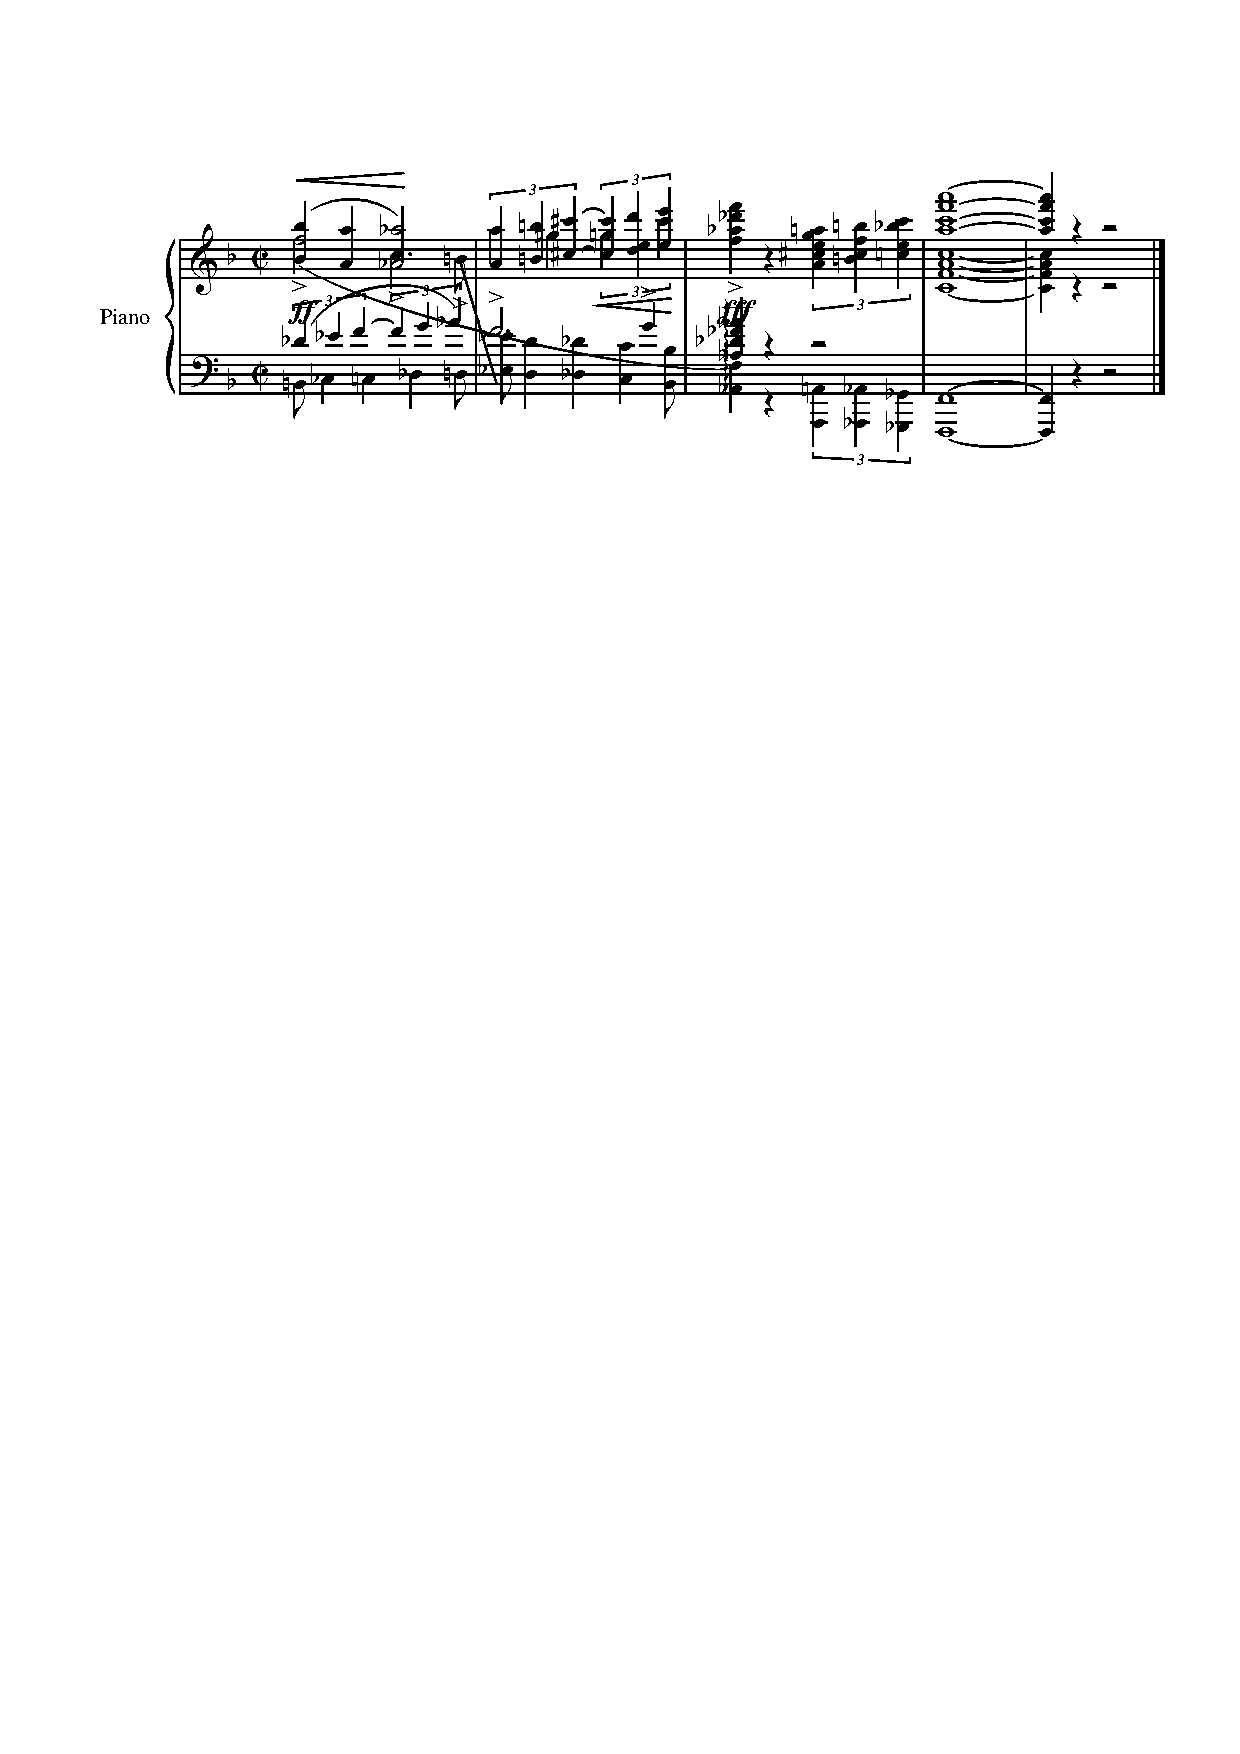
\includegraphics[width=19.5cm]{examples/schoenberg-opus-8-4-finale}


\end{document}